\documentclass[letterpaper,12pt]{article}
\usepackage[utf8]{inputenc}

\usepackage{graphicx}
\usepackage{csquotes}

\title{Data Science with Knowledge Graph \\{\large Literature Survey - part 2}}
\author{Shayan Amani}

\date{\today}

\begin{document}
\maketitle

\section{Introduction}
In this work, I review and study the literature on sentence and text generation using generative models. In the following three sections three recent papers on this topic are discussed. They have used generative models in nature to produce meaningful and syntactic text. Generative approaches based on convolutional neural networks (CNN) are more common in the literature. In a later section, I expand upon potential applications to TREC-CAR dataset.

\section{Generating Sentences from a Continuous Space}
Bowman et al. \cite{Bowman2015GeneratingSpace} proposed an RNN-based variational autoencoder generative model that incorporated distributed latent representations of entire sentences. Unlike vanilla RNN language models, this model worked from an explicit global sentence representation. Continuous sampling from the prior over these sentence representations produced diverse and grammatical sentences.

The recurrent neural network language model (RNNLM) \cite{MikolovExtensionsModel} generates sentences word-by-word based on an evolving distributed state representation and it does not expose a representation of high-level features such as syntactic properties or the topic. In \cite{Bowman2015GeneratingSpace} they proposed a variational autoencoder generative model as an extension of the RNNLM which is designed to explicitly capture such global features in a continuous latent variable. The variational autoencoder (VAE) \cite{Kingma2013Auto-EncodingBayes} is a generative model based on a regularized standard autoencoder. The VAE modifies the autoencoder architecture by replacing the deterministic function $\varphi_{enc}$ with a learned posterior recognition model, $q(\vec{z}|x)$ over hidden codes $\vec{z}$ using a neural network conditioned on $x$. Intuitively, the VAE learns codes not as single points, but as soft ellipsoidal regions in latent space, forcing the codes to fill the space rather than memorizing the training data as isolated codes.

\begin{figure}
    \centering
    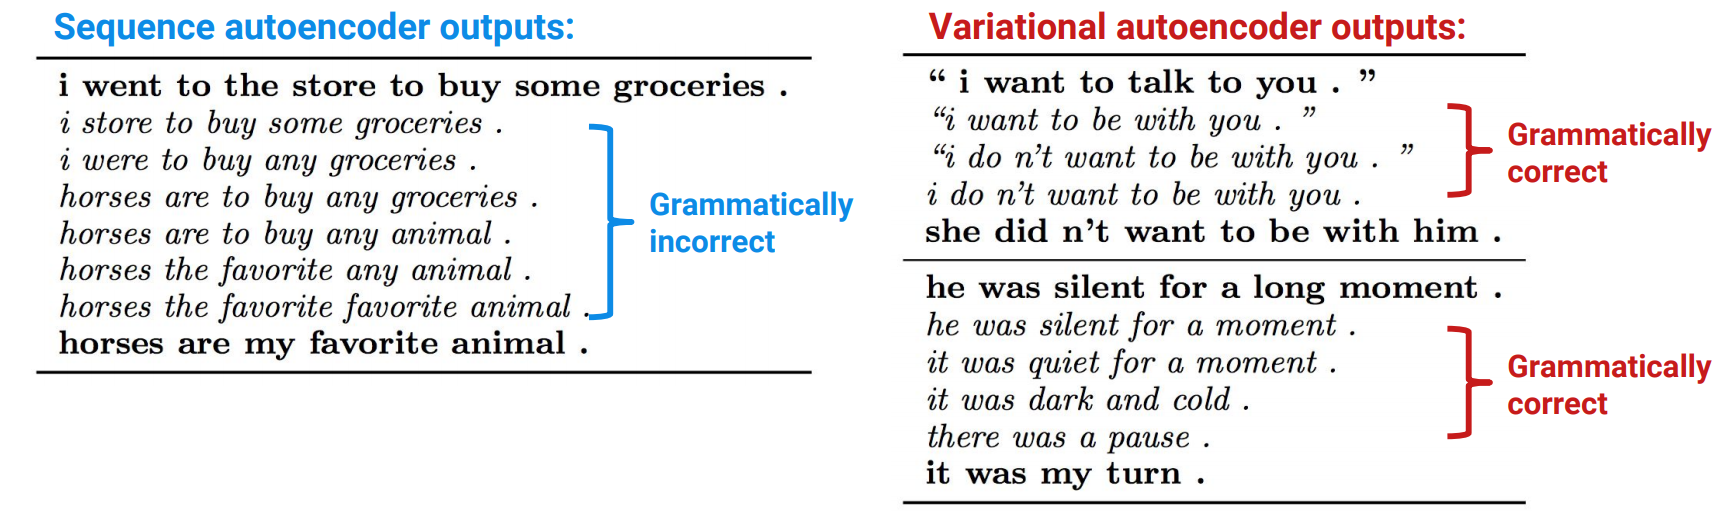
\includegraphics[width=\1\columnwidth]{literature_surveys2/seqAE-vs-VAE.png}
    \caption{A comparison between a sequence autoencoder's and a variational autoencoder's generated sentences}
    \label{fig:seqAE-vs-VAE}
\end{figure}

In order to generate sentences the authors adapted the variational autoencoder to text by using single-layer LSTM RNNs \cite{hochreiter1997a} for both the \textit{encoder} and the \textit{decoder}, essentially forming a sequence autoencoder with the Gaussian prior acting as a regularizer on the hidden code. The decoder serves as a special rnn language model that is conditioned on this hidden code, and in the degenerate setting where the hidden code incorporates no useful information, this model is effectively equivalent to an RNNLM. In figure \ref{fig:seqAE-vs-VAE}, I have used two homotopies (linear interpolation between sentences) available in the paper to illustrate generated sentences from two models in sentence generation.

\section{SeqGAN: Sequence Generative Adversarial Nets with Policy Gradient}
One problem with applying generative adversarial networks (GAN) to text is that the gradients from the discriminator cannot properly back-propagate through discrete variables. The Authors in \cite{Yu2016SeqGAN:Gradient} have proposed to bypass this problem by modeling the generator as a stochastic policy. The reward signal came from the GAN discriminator judged on a complete sequence, and was passed back to the intermediate state-action steps using Monte Carlo search.

The evaluation of deep generative models has been challenging. strategy is to evaluate bilingual evaluation understudy (BLEU) \cite{Papineni2002BLEU:Translation} scores of samples on a large amount of unseen test data. The ability to generate similar sentences to unseen real data is considered a measurement of quality.


\section{Generating Text via Adversarial Training}
 Zhang et al.\cite{Zhang2016GeneratingTraining} proposed a framework of generating realistic text, namely textGAN, in which the model uses feature distribution to train the generator. As in figure \ref{fig:textGAN}, the framework employ LSTM and CNN for adversarial training to generate realistic text. The latent code $z$ was fed to the LSTM generator at every time step. CNN acted as a binary sentence classifier which discriminated between real data and generated samples. One problem with applying GAN to text is that the gradients from the discriminator cannot properly back-propagate through discrete variables. In this paper, this problem was solved by making the word prediction at every time “soft” at the word embedding space.
 
 \begin{figure}
    \centering
    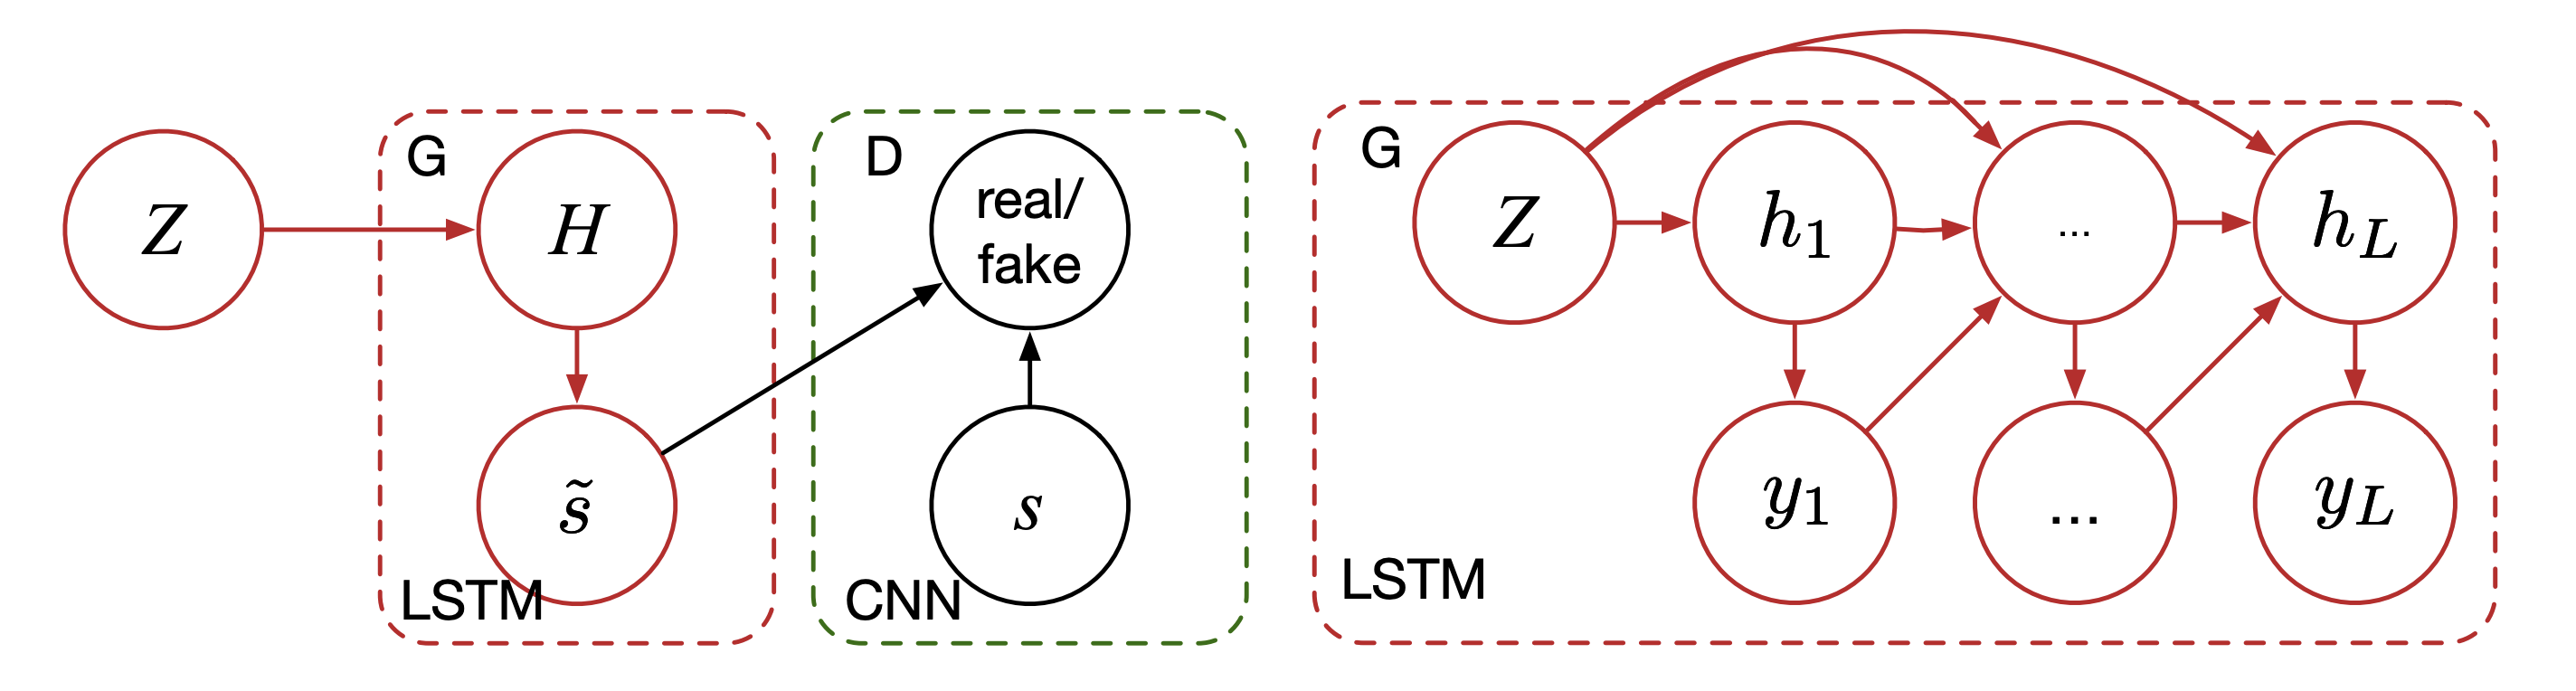
\includegraphics[width=\1\columnwidth]{literature_surveys2/textGAN.png}
    \caption{Left: Illustration of the textGAN model. The discriminator is a CNN, the sentence decoder is an LSTM. Right: the structure of LSTM model}
    \label{fig:textGAN}
\end{figure}

Standard sentence autoencoders, do not impose any constraint on the latent space, as a result, they fail when generating realistic sentences from arbitrary latent representations \cite{Bowman2015GeneratingSpace}. The authors clearly stated that the representations of such sentences may often occupy a small region in the hidden space and most of the regions in the hidden space do not necessarily map to a realistic sentence.


\section{Conclusion}
I have described three different papers on sentence generation models and pointed out their properties. TREC-CAR dataset \cite{dietz}, is an effort to retrieve longer answers with more information such as Wikipedia pages. Queries as input to the retrieval model have a major impact on the results. I have suggested my proposed area of application to improve the retrieval system. Query auto-completion which means suggesting complete and curated queries based on some initial words. Using the approach in \cite{Bowman2015GeneratingSpace}, a set of possible query sentences can be offered generated by intermediate non-grammatical combination of words. Through the model in \cite{Bowman2015GeneratingSpace}, a complete synthetic sentence is derived. By harnessing this advantage, we may even save user's time and also get a more semantically clear query which may yield an improvement in result measurements. Another possibility is producing a set of queries to benchmark different models. Queries from human are always along with biases. Generative models are able to generate versatile sentences from different points in the latent space. Next application could be suggesting a set of other queries which may the user is interested in. These generated sentences are the next point for further queries to retrieve even more information about a topic by expanding homotopies from the initial sentence to the generated ones. The proposed features are a set of enhancements that can be overseen in order to reach even more accurate information from TREC-CAR.


\bibliographystyle{nips}
\bibliography{library}

\end{document}